% Chapter 1
\chapter{State of the art} % Main chapter title
\label{Chapter1} % For referencing the chapter elsewhere, use \ref{Chapter1} 

\startcontents[chapters]
\Mprintcontents


%----------------------------------------------------------------------------------------

% Define some commands to keep the formatting separated from the content

%----------------------------------------------------------------------------------------

Forest are complex areas, the mapping of such environment needs the use of different image processing methods. The extraction of "homogeneous" forest stands is at the interplay between different kinds of image processing methods.

Several methods have been proposed for the forest stand segmentation (section \ref{sec:C1_stand}). They employ different image processing algorithms. Segmentation (section \ref{sec:C1_seg}) algorithms can be employed for a fine or coarse delineation of the principal components of the forests. Classification is also very useful to discriminate the different elements of the forest and detect tree species (section \ref{sec:C1_classif}). Furthermore, with the growing number of feature that could be derived, feature selection algorithms are mandatory in order to improve the results while decreasing the computational load and times (section \ref{sec:C1_fs}). Eventually, smoothing methods could be employed in order to obtain a minimum of an energy. Such energy minimization processes are used for a refinement of raw results (section \ref{sec:C1_smooth}).

\section{Stand segmentation}
\label{sec:C1_stand}
A forest stand is defined as a contiguous group of trees that are uniform in specie composition, structure, age and/or height, spatial arrangement, site quality or condition to distinguish it from adjacent other groups of trees.

One should note that the literature remains heavily focused on individual tree extraction and tree species classification \citep{dalponte2014tree, vega2014ptrees, kandare2014new}, developing site-specific workflows with similar advantages, drawbacks and classification performance. More authors have focused on forest delineation \citep{eysn2012forest, wang2012forest, radoux2007quantitative}, that most of the time do not convey information about the tree species and their spatial distribution. Even if some methods have proposed forest stand delineation, they remain very specific to the study area and provide a binary mask as final output. Consequently, no operational framework embedding the automatic analysis of remote sensing data has been yet proposed in the literature for forest stand segmentation at large scale \citep{clement_IJPRS}. \\

Hence, in the large amount of literature in the field, only few papers focus on the issue of stand segmentation or delineation. They can be categorized with regard to the type of data processed. \\
\subsection{Stand segmentation using VHR optical images}
A stand delineation technique using VHR airborne hyperspectral imagery is proposed in \citep{leckie2003stand}. The trees are extracted using a valley following approach and classified into 7 tree species (5 coniferous, 1 deciduous, and 1 non-specified) with a maximum likelihood classifier. A semi-automatic iterative clustering procedure is then introduced to generate the forest polygons.\\

A hierarchical and multi-scale approach for the identification of stands is adopted in \citep{hernando2012spatial}. The data inputs were the 4 bands of an airborne 0.5$\:$m orthoimage (Red, Green, Blue, and Near Infra-Red) allowing to derive the Normalized Difference Vegetation Index (NDVI). The stand mapping solution is based on the Object-Based Image Analysis concept. It is composed of two main phases in a cyclic process: first, segmentation, then classification. The first level consists in over-segmenting the area of interest and performing fine-grained land cover classification. The second level aims to transfer the vegetation type provided by a land cover geodatabase in the stand polygons, already retrieved from another segmentation procedure. The multi-scale analysis appears to have a significant benefit on the stand labeling but it is highly heuristic and requires a correct definition of the stand while we consider it is an interleaved problem. \\

Following the work of \citep{Wulder2008} with IKONOS images, Quickbird-2 panchromatic images are used in \citep{Mora20102474} to automatically delineate forest stands. A standard image segmentation technique is used and the novelty mainly lies on the fact that its initial parameters are optimized with respect to NFI protocols. They show that meaningful stand heights can be derived, which are a critical input for various modeled inventory attributes.\\

\subsection{Stand segmentation using lidar}
A seminal stand mapping method using low density airborne lidar data is proposed in \citep{koch2009airborne}. It is composed of several steps of feature extraction, creation and raster-based classification. Forest stands are created by grouping neighboring cells within each class. Then, only the stands with a pre-defined minimum size are accepted. Neighboring small areas of different forest types that do not reach the minimum size are merged together to an existing forest stand. The approach offers the advantage of detecting 15 forest types (deciduous/coniferous and maturity) that match very well with the ground truth but to the detriment of simplicity: the flowchart has to be highly reconsidered to fit to other stand specifications. Additionally, the tree species discrimination is not addressed.\\

The forest stand delineation proposed in \citep{sullivan2009object} also uses low density airborne lidar still coupling an object-oriented image segmentation and a supervised classification procedure. Three features are computed and rasterized. The segmentation is performed using a region growing approach. Spatially adjacent pixels are grouped into homogeneous discrete image objects or regions. Then, a supervised discrimination of the segmented image is performed using a Battacharya classifier, in order to determine the maturity of the stands. The tree species are ignored and the procedure requires a careful inspection of the raw data both for feature generation and model training. \\

The method proposed in \citep{eysn2012forest} aims to generate a forest mask (\textit{forested area} label only) using low density airborne lidar. A Canopy Height Model (CHM) with a spatial resolution of 1$\:$m is derived. The positions and heights of single trees are determined from the CHM using a local maximum filter, based on a moving window approach. Only detected positions with a CHM height superior to 3$\:$m are considered. The crown radii are estimated using an empirical function. The three neighboring trees are connected using a Delaunay triangulation applied to the previously-detected tree position. The crown cover is then calculated using the crown areas of three neighboring trees and the area of their convex hull for each tree triple. The forest mask is derived from the canopy cover values. While this is not a genuine stand delineation method, this approach could be easily extended to a multi-class problem and enlightens the necessity of individual tree extraction even with limited point densities as a basis for the stand-level analysis.\\

A forest stand delineation also based on airborne lidar data is proposed in \citep{wu2014data}. Three features are first directly extracted from the point cloud. A coarse forest stand delineation is then performed on the feature image using the unsupervised Mean-Shift algorithm, in order to obtain under-segmented raw forest stands. A forest mask is then applied to the segmented image in order to retrieve forest and non-forest raw stands. It may create some small isolated areas, iteratively merged to their most similar neighbor until their size is larger than a user-defined threshold in order to product big raw forest stands. They are then refined into finer level using a seeded region growing based on superpixels. The idea is to select several different superpixels in a raw forest stand and merge them. This method provides a coarse-to-fine segmentation with relatively large stands. The process was only applied on a small area of a forest in Finland, thus, general conclusions can not be drawn. \\

\subsection{Stand segmentation using VHR optical images and lidar}
The analysis of the lidar and multispectral data is performed at three levels in \citep{tiede2004object}, following a given hierarchical nomenclature of classes in forested environments. The first level represents small objects (single tree scale, individual trees or small groups of trees) that can be differentiated by spectral and structural characteristics using a rule-based classification. The second level corresponds to the stand level. It is built using the same classification process which summarizes forest development phases by referencing to small scale sub-objects at level 1. The third level is generated by merging objects of the same classified forest-development into larger spatial units. The multi-scale analysis offers the advantage of alleviating the standard issue of individual tree crown detection and proposing development stage labels. Nevertheless, the pipeline is highly heuristic, under-exploits lidar data and significant confusions between classes are reported.\\

The automatic segmentation process of forests in \citep{diedershagen2004automatic} is also supplied with Lidar and VHR multispectral images. The idea is to divide the forests into higher and lower sections with lidar. An unsupervised classification process is applied to the two images. The final stand delineation is achieved by segmenting the classification results with pre-defined thresholds. The segmentation results are improved using morphological operators such as opening and closing, which fill the gaps and holes at a specified extent. This method is efficient if the canopy structure is homogeneous and requires a strong knowledge on the area of interest. Since it is based on height information only, it cannot differentiate two stands of similar height but different species.\\

In \citep{leppanen2008automatic} a stand segmentation technique for a forest composed of \textit{Scots Pine}, \textit{Norway Spruce} and \textit{Hardwood} is defined. A hierarchical segmentation on the Crown Height Model followed by a restricted iterative region growing approach is performed on images composed of rasterized lidar data and Colored Infra-Red images. The process was only applied on a limited area of Finland and prevents from drawing strong conclusions. However, the quantitative analysis carried out by the authors shows that lidar data can help to define statistically meaningful stands (here the criterion was the timber volume) and that multispectral images are inevitable inputs for tree species discrimination. \\

\subsection{Challenges of stand segmentation}
Table~\ref{table:methods} summarizes the presented methods of forest stands segmentation. Firstly, it appears that the fusion of the remote sensing modalitie (optical images and lidar) improve the results for the problematic of forest stand delineation. However, the stands are not defined the same way in the different proposed methods, preventing from drawing general conclusion.
\begin{sidewaystable}[htbp]
\begin{center}
\begin{tabular}{|l|c|c|c|}
\hline
\textbf{Reference} & \textbf{Data processed} & \textbf{Country} & \textbf{Segmentation criteria} \\
\hline
\cite{leckie2003stand} & Hyperspectral images & Canada & Tree species (7) \\
\hline
\cite{hernando2012spatial} & Multispectral images & Spain & Vegetation type \\
\hline
\cite{Mora20102474} & Panchromatic images & Canada & Height \\
\hline
\cite{koch2009airborne} & Lidar & Germany & Forest types (15) \\
\hline
\cite{sullivan2009object} & Lidar & USA & Tree maturity \\
\hline
\cite{eysn2012forest} & Lidar &  Austria & Forest mask \\
\hline
\cite{wu2014data} & Lidar & Finland & Tree size, tree density \\
\hline
\cite{tiede2004object} & Lidar and multispectral images & Germany & Development phase \\
\hline
\cite{diedershagen2004automatic} & Lidar and multispectral images & Germany & Canopy structure, height \\
\hline
\cite{leppanen2008automatic} & Lidar and multispectral images & Finland & Tree species (3) \\
\hline
\end{tabular}
\caption{Existing methods for forest stand segmentation, see text for more details.}
\label{table:methods}
\end{center}
\end{sidewaystable}

Regarding the existing state of the art on the forest stand segmentation, it appears that such task is very complex to implement. Indeed, a simple segmentation (without semantic information) is not sufficient since it does not allows to retrieve consistent stands. A classification is mandatory in order to obtain the tree species. However, it is very difficult to discriminate species, since some have a very close looking (e.g. deciduous oak and beech), and the intra-class variability might be important (depending on age, maturity). Eventually, the desired stands are not totally pure, a certain level of generalization is desired in order to have a consistent mapping at large scale. Thus, a regularization process can be employed for such purpose.
It also appears that the type of data employed has an impact on the results.
\begin{itemize}
\item The VHR optical images permits to obtain information about the tree species, especially when using textural features \citep{franklin2000incorporating}.
\item The lidar data provides information about the vertical structure of the forest that can also be useful for the discrimination of tree species \citep{brandtberg2007classifying}. It also brings information about the height that allows to separate forest stands of different ages. Most of the time, lidar is deeply under exploited since it is used only as a simple DSM.
\end{itemize}

\section{Segmentation}
\label{sec:C1_seg}
The direct segmentation of optical image and/or lidar point clouds is not sufficient in order to retrieve forest stands. Indeed, such segmentation methods can not take into account the information needed to define the stand.  However, with adapted parameters, segmentations algorithms might be useful to obtain relevant segmentation of the data \citep{clement_IJPRS}. They can be divided in two categories:
\begin{itemize}
\item The "traditional" segmentation methods; in these methods, a specific attention must be paid to the choice of the parameters in order to obtain relevant results. Such segmentation can be applied on an image or a point cloud. Specific methods have also been developed for the segmentation of lidar point cloud \citep{nguyen20133d}.
\item The superpixels segmentation methods: they natively produce an over-segmentation of the image. The parameters control the size and the shape of the resulting segments.
\end{itemize}

\subsection{"Traditional" segmentation methods}
The segmentation of an image can be performed using a large variety of techniques \citep{wilson1988image, nitzberg1993filtering, pal1993review, zhang2006advances}. \\

The easiest way to segment an image is the thresholding of a gray level histogram of the image \citep{taxt1989segmentation}. When the image is noisy or the background is uneven and illumination is poor, such thresholding is not sufficient. Thus, adaptive thresholding methods have been developed \citep{yanowitz1989new}. \\

The watershed transformation is also a simple segmentation method that considers the gradient magnitude of an image as a topographic surface. Pixels having the highest gradient magnitude intensities correspond to watershed lines, which represent the region boundaries. Water placed on any pixel enclosed by a common watershed line flows downhill to a common local intensity minimum. Pixels draining to a common minimum form a catch basin, which represents a segment.

The segmentation can be considered as an unsupervised classification problem. Algorithms dealing with such problems adopt iterative process. The most popular algorithm is the k-means algorithm. Segmentation methods using the spatial interaction models like Markov Random Field (CRF) \citep{hansen1982image} or Gibbs Random Field (GRF) \citep{derin1987modeling}. Neural networks are also interesting for  image segmentation \citep{ghosh1991image} as they take into account the contextual information. \\

The segmentation of an image can also be obtained by the detection of the edges of the image \citep{peli1982study}. The idea is to extract points of significant changes in depth values. Edges are local features and are determined based on local information. \\

Eventually, hierarchical segmentation algorithms can be employed. They analyze simultaneously the image at several different scales of analysis. Their output is not a single partition, but a hierarchy of regions or data structure that captures different partitions for different scales of analysis \citep{trias2006semi, guigues2006scale, baatz2004method}. These methods allow to control the complexity of the segmentation, which was not the case for the previous methods. The algorithm is a bottom-up approach that starts with an initial over-segmentation (e.g. segmenting almost each pixel on a different own region) and uses this level as a base for the construction of subsequent significant levels. The segmentation process is guided by an energy $E$ of the form:
\begin{equation}
E = D + \mu C
\end{equation}
where, $D$ is a fit-to-data measure (how well the segmentation fits to the original image, better fits give lower values of $D$); $C$ is a measure of segmentation complexity (less complex solutions give lower values of $C$); and $\mu$ is a dimensional parameter, the scale parameter. The parameter $\mu$ balances between a perfect fit to the original data ($\mu=0$), consisting of one segmentation region for each pixel in the original image, and the simplest segmentation, consisting of a single region containing the whole image \citep{guigues2006scale} (see Figure~\ref{fig:seg_hierar}). The level of segmentation can be adjusted gradually from the finest to the coarsest depending of the image complexity.

\begin{figure}[htbp]
\begin{center}
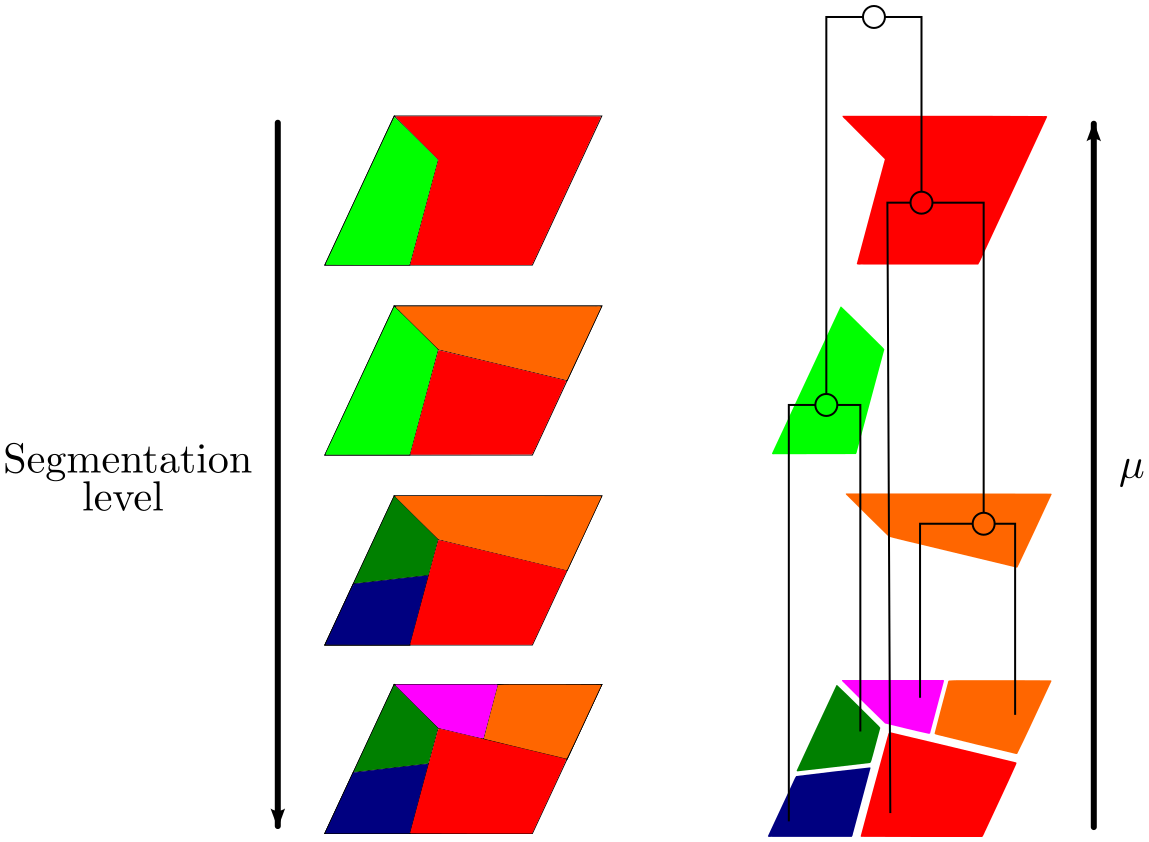
\includegraphics[width=0.75\textwidth]{Figures/seg_hierar}
\caption{Graphical depiction of concepts related to hierarchical segmentation. The diagram on the left shows partitions of an image at four different scales $\mu$. The partition at the top has the highest $\mu$ and is therefore the coarsest, the partition at the bottom is the finest.}
\label{fig:seg_hierar}
\end{center}
\end{figure}

Top-down approaches can also be employed for image segmentation. In \cite{landrieu2016cut} working-set/greedy algorithms to efficiently solve problems penalized respectively by the total variation on a general weighted graph are proposed. The algorithms exploit this structure by recursively splitting the level-sets of a piecewise-constant candidate solution using graph cuts.

\subsection{Superpixels methods}
Several superpixels algorithms have been developed \citep{achanta2012slic}. They group pixels into perceptually meaningful atomic regions. Many traditional segmentation algorithms have been employed with more or less success to generate superpixels \citep{shi2000normalized, felzenszwalb2004efficient, comaniciu2002mean, vedaldi2008quick, vincent1991watersheds}. These algorithms produce satisfactory results, however, they may be relatively slow and the number, size and shape of the superpixels might not be specified. \\

Superpixels algorithms have then been developed. One can control the number of superpixel, their size and their shape. \cite{moore2008superpixel} creates superpixels based on a grid. Optimal path are found using graph cut methods. \cite{veksler2010superpixels} proposes a generation of superpixels based on a global optimization. They are obtained by stitching together overlapping image patches such that each pixel belongs to only one of the overlapping regions. \cite{levinshtein2009turbopixels} generate superpixels by a dilatation of a set of seed locations using level-set geometric flow. Resulting superpixels are constrained to have uniform size, compactness, and boundary adherence. Finally, \cite{achanta2012slic} proposes a generation of superpixels based on the k-means algorithms. A weighted distance that combines color and spatial proximity is introduced in order to control the size and the compactness of the superpixels.


\subsection{Segmentation of point cloud}
The segmentation of point cloud has been highly assessed \citep{nguyen20133d}. The aim is to extract meaningful objects. Such extraction has two principal objectives:
\begin{itemize}
\item Objects are detected so as to ease or strengthen subsequent classification task. A precise extraction is not mandatory since the labels would be refined after.
\item Objects are precisely delineated in order to derive features from these objects. A high spatial resolution is therefore expected.
\end{itemize}

In forested areas, the only reliable objects to extract are trees. The first way to extract trees from lidar data is to rasterize the point cloud and use image-based segmentation techniques to obtain trees. Several methods have been developed for single tree delineation \citep{dalponte2014tree, vega2014ptrees, kandare2014new}. 

\section{Classification}
\label{sec:C1_classif}
A classification is a process that aims to categorize observation. The idea is to assign an observation to one or more classes. This can be done manually or automatically. The classification can be unsupervised, the classes need to be learned and the observation assigned. Such classification is similar to segmentation (see section \ref{sec:C1_seg}). The classification can be supervised, the target classes are known and observations with labels are available.

\subsection{Supervised classification}
A great number of supervised classification algorithms have been developed and used for remote sensing issues \citep{landgrebe2005signal, lu2007survey, mather2016classification}. There are two kind of algorithms: the parametric (or generative) and the non-parametric (or discriminative) methods.

The parametric method assume that each class follow a specific distribution (mainly gaussian). The parameters of the distribution are estimated using the learning set. This is the case for the maximum likelihood \citep{strahler1980use}, maximum a posteriori \citep{fauvel2015fast} or in \cite{trias2005high}.

The non parametric methods do not make any assumption on the classes distribution. In this category of algorithms, the most popular are the Support Vector Machines (SVM) \citep{boser1992training, scholkopf2001learning} and the Random Forest (RF) \citep{breiman2001random}. The artificial neural networks are also efficient algorithms \citep{hepner1990artificial, atkinson1997mapping}. However, despite their great performance in terms of accuracy, they have several drawbacks: firstly, the training process is time consuming and good GPU cards or specific architectures are required in order to reach decent training times \citep{dean2012large, moritz2015sparknet}. Secondly, it requires an important amount of training data in order to correctly optimize the large number of parameters (e.g., hundred of millions). Simpler methods exist, such as the k-nearest neighbor \citep{indyk1998approximate} or the decision trees \citep{breiman1984classification}. The non parametric methods are more efficient  for the discrimination of complex classes \citep{paola1995review, foody2002status}, and are considered as a basis for land cover classification \citep{camps2009kernel}.

We chose to use the RF, which besides their widespread use, since they also offer the possibility of obtaining the probability of belonging of a pixel to a class. This posterior probabilities can be then integrated into a smoothing process. They also report good results, similar to SVM (see Chapter~\ref{Chapter3}). The RF are described in section~\ref{sec:C1_RF}.

\subsection{Random Forest}
\label{sec:C1_RF}
The RF have been introduced by \cite{breiman2001random} and are defined by the aggregation of predictors (decision trees). Here, we refer to the RF with random inputs proposed in \cite{breiman2001random}.

The idea is to create an ensemble of samples $\mathcal{S}_{n}^{\Theta_{1}}$, ..., $\mathcal{S}_{n}^{\Theta_{k}}$ from an initial training set. A Classification and Regression Tree (CART) \citep{breiman1984classification} is built on each sample $\mathcal{S}_{n}^{\Theta_{i}}$. Each tree is built using a a random pool of $m$ features among the $M$ available features. The final classification is obtained by majority vote; each tree votes for a class and the class reaching the most votes wins (see Figure \ref{fig:RF_method}). This algorithm has two parameters: the number of trees $k$ and the number of features $m$ used to build a tree. The first parameter is arbitrary fixed to a high value. The second is generally fixed to the square root of the total number of feature \citep{gislason2006random}.

\begin{figure}[htbp]
\begin{center}
\begin{tikzpicture}
	[shape=circle,cap=round,scale=1]
	%
	\draw (0,2.5)  node[myNodeIGNGris] (data) {Dataset};
	\draw (-4,0.5)  node[myNodeIGNVert] (bootstrap1) {$\mathcal{S}_n^{\Theta_1}$};
	\node (ldots) at (0,0.5) {\textbf{\ldots}};
	\draw (4,0.5) node[myNodeIGNVert] (bootstrapN) {$\mathcal{S}_n^{\Theta_k}$};	
	
	\draw[thick,color=gray,rounded corners](-6.75,-5)--(-6.75,-1)--(-1.25,-1)--(-1.25,-5)--cycle;
	\node[color=gray] at (-5.25,-1.5) {CART 1};
	\node (first tree) at (-4,-3) {\tikz{%
	\node[draw,top color=blue!10,bottom color=blue,minimum size=6pt,circular drop shadow] {} 
	 child  foreach \A in {red,red,red}{  
	   node[draw,top color=\A!10,bottom color=\A,minimum size=4pt,circular drop shadow] {} 
	     child foreach \B in {green,green}{
	       node[draw,top color=\B!10,bottom color=\B,minimum size=3pt,circular drop shadow] {} 
	    }%
	 };%
	}};%
	
	\draw[thick,color=gray,rounded corners](1.25,-5)--(1.25,-1)--(6.75,-1)--(6.75,-5)--cycle;
	\node[color=gray] (cartk) at (2.75,-1.5) {CART K};
	\node (second tree) at (4,-3) {\tikz{%
	\node[draw,top color=blue!10,bottom color=blue,minimum size=6pt,circular drop shadow] {} 
	 child  foreach \A in {red,red,red}{  
	   node[draw,top color=\A!10,bottom color=\A,minimum size=4pt,circular drop shadow] {} 
	     child foreach \B in {green,green}{
	       node[draw,top color=\B!10,bottom color=\B,minimum size=3pt,circular drop shadow] {} 
	    }
	 };
	}};
	
	\draw (0,-6.5)  node[myNodeIGNGris] (vote) {Majority vote};
	
	\draw[myArrowIGNGris] (data.south) -- (0,1.5) -- (-4,1.5)  -- (bootstrap1.north);
	\draw[myArrowIGNGris] (data.south) -- (0,1.5) -- (4,1.5)  -- (bootstrapN.north);
	
	\draw[myArrowIGNGris] (bootstrap1.south) -- (-4,-1);
	\draw[myArrowIGNGris] (bootstrapN.south) -- (4,-1);
	
	\draw[myArrowIGNGris] (-4,-5) -- (-4,-5.5) -- (0,-5.5)  -- (vote.north);
	\draw[myArrowIGNGris] (4,-5) -- (4,-5.5) -- (0,-5.5)  -- (vote.north);

\end{tikzpicture}
\end{center}
\caption{General diagram of the operation of the Random Forest}
\label{fig:RF_method}
\end{figure}


RF have shown better classification performances than traditional Boosting methods \citep{breiman2001random} or SVM \citep{pal2005random}. They are also able to handle big dataset with large number of feature. Furthermore, a measure of feature importance have been introduced in \cite{breiman2001random}. It allows to qualify the relevance of the feature in the classification process \citep{strobl2007bias}.

The importance of a feature $\mathbf{X}_{j}$, $j\in\{1,...,q\}$ (with $q$ the number of feature) is defined as follow. Let $\mathcal{S}_{n}^{\Theta_{i}}$ be a ensemble of sample and $OOB_{i}$ all the observations that does not belong to $\mathcal{S}_{n}^{\Theta_{i}}$. $errOOB_{i}$, the error on $OOB_{i}$ using $\mathcal{S}_{n}^{\Theta_{i}}$, is then computed. A random permutation on the value of the $j^{\text{th}}$ feature of $OOB_{i}$ is performed in order to obtain $\widetilde{OOB_{i}}^j$. $err\widetilde{OOB_{i}^{j}}$ is then computed. The importance of the feature $j$, $FI(\mathbf{X_{j}})$ is the mean of the difference of the errors (see Equation \ref{eq:FI}).

\begin{equation}
\label{eq:FI}
FI(\mathbf{X_{j}})=\frac{1}{k}\sum_{i=1}^{k}(err\widetilde{OOB_{i}^{j}}-errOOB_{i})
\end{equation}
where $k$ is the number of CART.


\section{Dimension reduction and feature selection}
\label{sec:C1_fs}
It is possible to derive a lot a features from the original data. All the features are used for the classification. The feature selection methods try to overcome the curse of high dimensionality \citep{bellman2015adaptive, hughes1968mean}. Indeed, the increasing number of features available tends to decrease the accuracy of the classifiers. Furthermore, the computation times increase with the number of features. Thus, reducing the feature dimension is beneficial for the classification task.

Two kind of approaches exist: first the ones based on the extraction of new features summarizing the information by the transformation of the data, generally using a projection in a space of lower dimensionality. Secondly, feature selection approaches that aim to search for an optimal subset of the features.

\subsection{Dimension reduction: feature extraction}
The most popular dimension reduction method is the Principal Component Analysis (PCA). It is an unsupervised method that aim to maximize the variance between data \citep{jolliffe2011principal}. However, it has been demonstrated that PCA is not optimal for the purpose of classification \citep{cheriyadat2003principal}. Other methods have been developed based on the PCA: the Independent Component Analysis (ICA) \citep{jutten1991blind} maximizes the statistical independence between data, and the Maximum Autocorrelation Factor (MAF) \citep{larsen2002decomposition} maximizes the spatial auto-correlation. When training samples are available, supervised methods exist, such as the linear discriminant analysis (LDA) that tries to maximize both the intra-class homogeneity and the inter-class variance \citep{fisher1936use, lebart1997multidimensional}.

\subsection{Feature selection}
Feature selection aims to search for an optimal subset of features without modifying them. To obtain such subset, one can explore the subsets of features or define a criteria to evaluate the subsets. Furthermore, the selection can be supervised or unsupervised. The first aims to discriminate the better the classes while the second are looking for an optimal subset that contains the most informative and less redundant features.
Many exploration methods for feature selection have been proposed in the literature. The naive exhaustive exploration of all the subsets can be envisaged when the number of features is not important. 

\subsubsection{Existing methods}
The feature selection methods can be separated into 3 categories: filters, wrapper and embedded. Within the filter methods, one can distinguish the supervised and unsupervised case depending on whether the notion of classes is taken into account or not.

\paragraph{\underline{$\bullet$ Filters} \\}
The filters methods use a feature selection criteria independent from the classifier. They consider the features according to their capacity to bring together elements of the same class and separate the different elements \citep{john1997enhancements} Thus, these methods compute an individual importance score for each feature, classify the features according to this score and keep only the best. Such scores can be computed using training sample or not. Such methods are independent from a classifier and are used as preliminary step to classification. When training samples are available, separability measures (e.g., Fisher \citep{fisher1936use}, Bhattacharrya or Jeffires-Matusia) allow to determine whether a feature or a subset of feature is well adapted to discriminate the classes \citep{bruzzone2000technique, herold2003spectral, de2005band, serpico2007extraction}. Statistical measures derived from information theory such as the divergence, the entropy or the mutual information have been proposed in the unsupervised case \citep{martinez2007clustering, le2011constrained} or supervised case \citep{battiti1994using, guo2008fast, estevez2009normalized, sotoca2010supervised, cang2012mutual}.
To summarize, criteria for filter selection methods are numerous and cover different approaches. The supervised ones, which sort features according to an individual importance score and retain only the $n$ best remain limited since they do not take into account the dependencies between the selected features. Approaches that directly associate relevance scores with feature sets are more interesting. A distinction is made between supervised and unsupervised approaches. The unsupervised criteria are interesting, but present a risk of selecting attributes that would not all also be useful for classification.

\paragraph{\underline{$\bullet$ Wrapper} \\}
The wrapper methods weight the features according to their pertinence for the prediction \citep{kohavi1997wrappers}. This weighting is related to the performance of a classifier.  \cite{estevez2009normalized, li2011effective, yang2007research, zhuo2008genetic} propose approaches with SVM classifiers. \cite{zhang2007dimensionality, fauvel2015fast} use maximum likelihood classifiers. The RF is also employed in \cite{diaz2006gene}. Data are separated into two subset. The first is used for the training, while the second for the evaluation. The use of a classifier is a big advantage as it fits more to the envisaged problem but can lead to overfitting. However, the use of a classifier significantly increases the computation times. Furthermore, worse results could be obtained when using a feature subset with an other classifier.

\paragraph{\underline{$\bullet$ Embedded} \\}
Eventually, the embedded methods also involve a classifier and select the features during the training process \citep{tang2014feature}. They have two advantages: since they use the data as training, they are robust. Furthermore, the feature selection and the classification are performed together, thus, they are faster than the wrapper methods. Many methods have been proposed. The RF allow to assess the feature importance \citep{breiman2001random} an is also natively embedded since the irrelevant features will not be used in the classification process. Other methods are based on the SVM classifiers, the SVM-RFE (Recursive Feature Elimination) \citep{tuia2009classification} recursively removes the less pertinent features according to a weight estimated with a SVM.

\subsubsection{Optimize the selection}
The set of possible solutions is generally too large to be visited entirely. Thus, using heuristic rules allows to find a solution close enough to the optimal solution while visiting only a reasonable number of configurations. These optimization methods can generally be distinguished in sequential or incremental methods and stochastic methods.

\paragraph{\underline{$\bullet$ Sequential approaches} \\}
The first idea is to add features step by step (forward approaches), also called Sequential Forward Selection (SFS) \citep{marill1963effectiveness}. It could also be methods that start from the entire feature set and remove feature step by step (backward approaches), also called Sequential Backward Selection (SBS) \citep{whitney1971direct}. A generalization of these methods have been proposed in \cite{kittler1978feature}. Finally, the forward and backward methods could be combined in order to improve the process. The Sequential Floating Forward Selection (SFFS) and the Sequential Floating Backward Selection (SFBS) \citep{pudil1994floating} propose such improvement. \\

\paragraph{\underline{$\bullet$ Stochastic approaches} \\}
Stochastic algorithms will involve hazard in their exploration of the space of solutions. The random initialization and search for a solution can therefore propose different solutions of equivalent quality from a single dataset.
The generation of the subset can be totally random \citep{liu1997feature}. Genetic algorithms propose a ponderation of the subsets according to their importance \citep{goldberg1989genetic}. They allow a faster convergence to a more stable solution. The Particle Swarm Optimization (PSO) algorithm \citep{yang2007research}  is also a fast and select relevant features. For finding an approximate optimal subset of features,  simulated annealing \citep{de2005band, chang2011parallel}. \\

\section{Smoothing methods}
\label{sec:C1_smooth}
Pixel-wise classification is not sufficient for both accurate and smooth land-cover mapping with VHR remote sensing data. This is particularly true in forested areas: the large intra-class and low inter-class variabilities of classes result in noisy label maps at pixel or tree levels. This is why various regularization solutions can be adopted from the literature (from simple smoothing to probabilistic graphical models).\\
According to \cite{schindler2012overview}, both local and global methods can provide a regularization framework, with their own advantages and drawbacks.

\subsection{Local methods}
In local methods, the neighborhood of each element is analyzed by a filtering technique. The labels of the neighboring pixels (or the posterior class probabilities) are combined so as to derive a new label for the central pixel. Majority voting, Gaussian and bilateral filtering can be employed if it is not targeted to smooth class edges. The majority vote can also be used when a segmentation is available: the majority class is assigned to the segment.\\
The probabilistic relaxation is an other local smoothing method that aims at homogenizing probabilities of a pixel according to its neighboring pixels. The relaxation is an iterative algorithm in which the probability at each pixel is updated at each iteration in order to have it closer to the probabilities of its neighbors \citep{Gong198933}. It reports good accuracies with decent computing time and offers an alternative to edge aware/gradient-based techniques that may not be adapted in semantically unstructured environments.

\subsection{Global methods}
Global methods consider the full area of interest at the same time. They are based on Markov Random Fields (MRF, see Figure~\ref{fig:graph_cut}), the labels at different locations are not considered to be independent. The optimal configuration of labels is retrieved when finding the Maximum A Posteriori over the entire field \cite{Gab_MRF}. The problem is therefore considered as the minimization procedure of an energy $E$ over the full image $I$. Despite a simple neighborhood encoding (pairwise relations are often preferred), the optimization procedure propagates over large distances. Depending on the formulation of the energy, the global minimum may be reachable. However, a large range of optimization techniques allow to reach local minima close to the real solution, in particular for random fields with pairwise terms \cite{kolmogorov2004energy}. For genuine structured predictions, in the family of graphical probabilistic models, Conditional Random Fields (CRF, see Figure~\ref{fig:graph_cut}) have been massively adopted during the last decade. Interactions between neighboring objects, and subsequently the local context can be modeled and learned. In particular, Discriminative Random Fields (DRF, \cite{DRF}) are CRF defined over 2D regular grids, and both unary/association and binary/interaction potentials are based on labeling procedure outputs. Many techniques extending this concept or focusing on the learning or inference steps have been proposed in the literature \cite{ijcv_kohli09,Ladicky2012}. A very recent trend even consists in jointly considering CRF and deep-learning techniques for the labeling task \cite{CNN_CRF}.\\

\begin{figure}[htbp]
\begin{center}
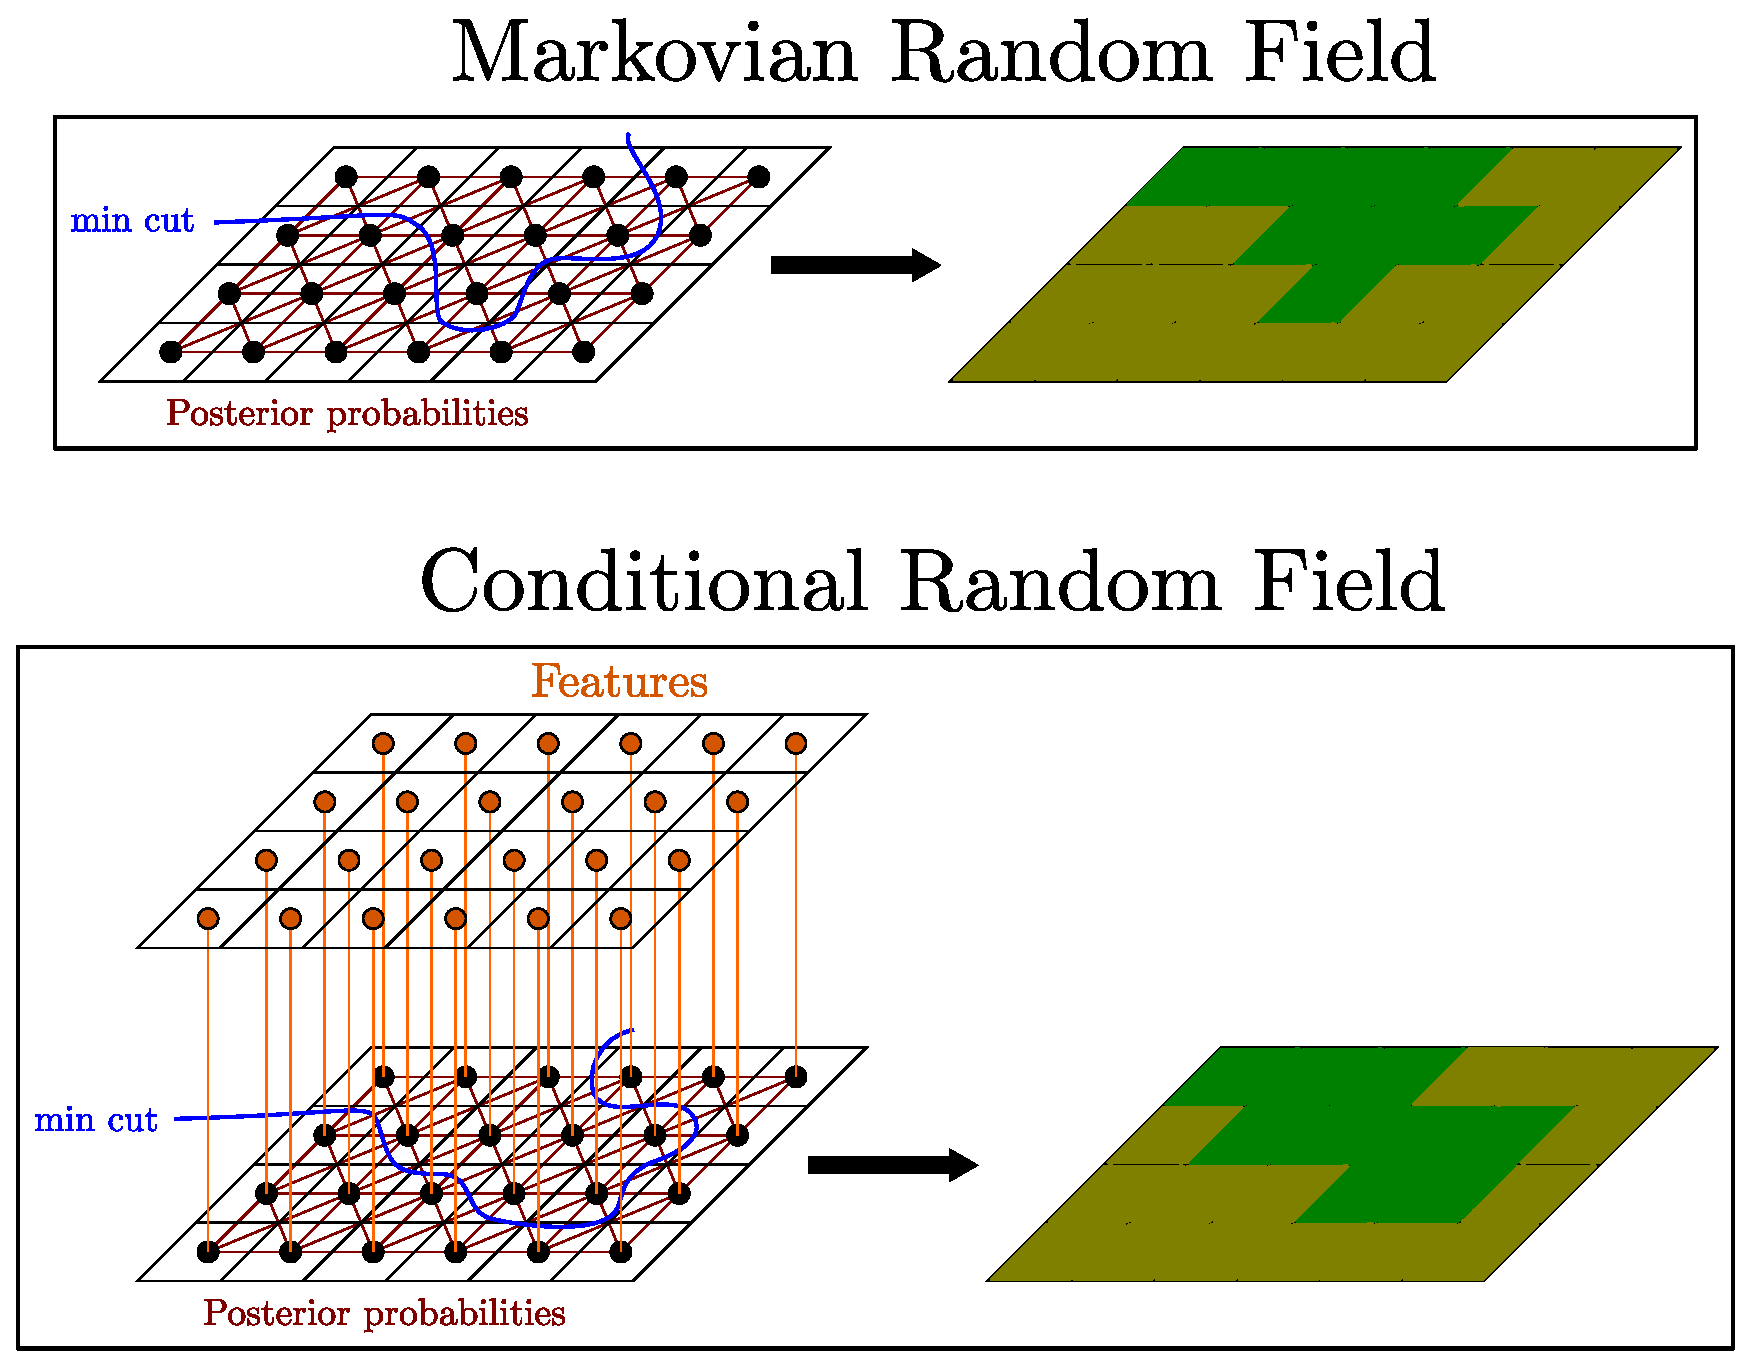
\includegraphics[width=\textwidth]{Figures/graph_cut}
\caption{8-connected MRF and CRF. The MRF only take into account the posterior probabilities to compute the graph, while CRF also include contextual information (the features).}
\label{fig:graph_cut}
\end{center}
\end{figure}

In standard LC classification tasks, global methods are known to provide significantly more accurate results \cite{schindler2012overview} since contextual knowledge is integrated. This is all the more true for VHR remote sensing data, especially in case of a large number of classes (e.g., 10, \cite{isprs-archives-XLI-B4-11-2016}), but presents two disadvantages. For large datasets, their learning and inference steps are expensive to compute. Furthermore, parameters should often be carefully chosen for optimal performance, and authors that managed to alleviate the latter problem still report a significant computation cost \cite{Lucchi_ICCV2011}.

\stopcontents[chapters]

